\section{理论机制探究}

小鼠和人的行为学实验结果都显示了,对于规律性时间间隔的刺激,
被试需要对其进行一定的学习和适应过程。尤其是对于人的实验结果,
我们可以看到被试通常在前四个刺激(第一个五份)内就已经能够较为
准确的预测我们设定的时间间隔了。我们可以将这一学习过程看作是
强化学习(reinforcement learning)的过程: 每次光栅刺激小鼠都会
得到相应的水作为反馈,而人则可以直接将是否正确完成任务作为反馈
来调整自己的行为。

学习的过程通常与突触间的可塑性相关联,而人的学习过程十分短暂,
提示可能与短时程突触可塑性(STP)有关;而小鼠的行为在七天训练中
逐渐好转,提示其学习过程可能与长时程突触可变性(LTP)相关。
而在感觉皮层中,最重要的一类兴奋性神经元是锥体神经元(Pyramidal neuron),
其最大的特点在于树突可以分为两大部分,即尖端树突(apical dendrites)和
基树突(basal dendrites)。其尖端树突通常接受来自其他脑区的投射,
而基树突主要与周围神经元进行交流,而突触棘在树突上的空间分布通常决定着
神经元的选择性\cite{mel2017synaptic}。
突触后电位在树突上的整合通常是非线性的,
也有实验研究表明尖端树突对胞体的放电主要其调制(modulation)的作用,
而基树突接受的信号才是决定胞体放电特异性的主要因素\cite{caze2017dendrites,branco2011synaptic}。
尖端树突接受的来源往往十分广泛而复杂,有实验表明其来源除了与其相关
的感觉输入外,还与刺激相关的时间信息,对刺激的预测,刺激后的反馈(奖赏)
等多种因素相关\cite{lacefield2019reinforcement}。

脑电信号的能量通常可以与该区域内神经元的发电强弱相对应。
而患者在空想范式下脑电信号能量也有上升,但幅度较其他两种范式小(图\ref{fig:ephys_network}~a)。
这可能是由于来自其他脑区的信号在注意力减弱是也相应减弱,通过
尖端突触的调制作用而产生的。但具体的机制仍需要更详尽的实验加以验证。

然而,脑电信号的相位很难和生物学上的意义相对应,而只能抽象的认为是该区域内
神经元放电的某种模式或状态。在患者轻拍手的范式下,提前打手和延后打手的
脑电信号相位有着明显的不同(图\ref{fig:ephys_network}~c)。
这可能是由于只有视觉刺激时,神经元放电不是很协调;而当与预测相关的信号
同时到达尖端突触时,神经元的放电会被协调而呈现一定的模式(图\ref{fig:theory})。

\begin{figure}[h]
    \centering
    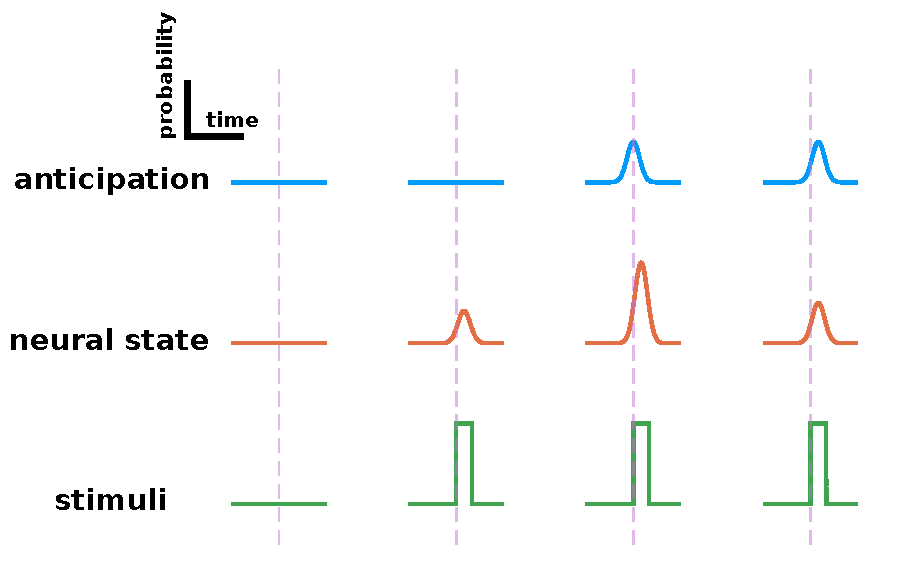
\includegraphics[width=\textwidth]{src/figures/theory.pdf}
    \caption{\textbf{可能的理论机制}\\
    在最初还没有学会时间间隔时,被试对刺激没有预测,如第二列所示。
    学会时间间隔后,若正确做出预判,神经元的状态可能会较没有预测时不同,如第三列所示。
    倘若预测出现失误,则神经元的状态可能而学习前类似,如第四列所示。}
    \label{fig:theory}
\end{figure}

